\documentclass{llncs}

% TODO:
% 10 oages
% Because there are no publications about external atoms in Alpha, we may reference DLV-Hex and say that external
% atoms are supported in a similar manner.
%
% A little example showcasing external atoms should be provided.
%
% Formalize "down lifting" of higher order predicates and describe it.
% Its probably is fair to introduce ASP.

\usepackage[utf8]{inputenc}
\usepackage[T1]{fontenc}

\usepackage{hyperref}
\usepackage{graphicx}

% Needs splncs03.bst via Springer
\bibliographystyle{splncs03}

\usepackage{amsmath, amssymb} % For \flalign, \top, ...
\usepackage[ruled,linesnumbered]{algorithm2e}

\usepackage[table,usenames,dvipsnames]{xcolor}
\usepackage{nicefrac,xspace,csquotes}

\newcommand{\fail}{\mathrm{not } \ \xspace}
%\newcommand{\from}{\mathrm{\ \xspace :- \ \xspace}}
\newcommand{\from}{\ensuremath{\leftarrow}}

\newcommand{\entails}{\models}

% Least model (of a Horn program).
\newcommand{\lm}{\mathrm{lm}}

% Set of stable models (of a program).
\newcommand{\stm}{\mathrm{STM}}
\newcommand{\sol}{\mathrm{Sol}}
\newcommand{\compl}{\mathrm{Co}}
\newcommand{\groundext}{\mathrm{Gr}}
\newcommand{\defense}{\mathrm{Def}_F}

% Entails according to well founded semantics.
\newcommand{\wf}{\ensuremath{\entails_{wf}}}

% Entails according to stable model semantics using brave reasoning
\newcommand{\brave}{\ensuremath{\entails_{st}^b}}

% Entails according to stable model semantics using cautious reasoning
\newcommand{\caut}{\ensuremath{\entails_{st}^c}}

% Selective Linear Definite-clause with Negation as Failure
\newcommand{\sldnf}{\ensuremath{\vdash_{NF}}}

\newcommand{\universe}{\mathcal{U}}
\newcommand{\afs}{\mathcal{F}}
\newcommand{\attacks}{\rightsquigarrow}

\newcommand{\ah}{Angry-HEX\xspace}
\newcommand{\al}{Alpha\xspace}

\title{Complex Predicates~vs.~Complex Objects}
\subtitle{A Case Study on Answer Set Programming\\ for Implementing Artificial Agents}
\author{Filippo~De~Bortoli \and Lorenz~Leutgeb \and Cosimo~Damiano~Persia}
\institute{International Center for Computational Logic, TU Dresden\\ \texttt{\{{filippo.de\_bortoli,lorenz.leutgeb,cosimo\_damiano.persia\}\newline @mailbox.tu-dresden.de}}}

\begin{document}

\maketitle

\begin{abstract}
Angry Birds is a 2D video game in which objects are hurled at targets using a slingshot in order to score points. The game sparked interest in the research community and a variety of agents have been developed.
In the fashion of a case study, this work considers on of these agents, namely \ah, which reasons about playing strategy and tactics using \emph{Answer Set Programming} (ASP), a well established formalism for \emph{Knowledge Representation and Reasoning} (KRR).
In order to interface with the game (a web application), and to integrate simulation of physics into the reasoning process, the implementation of \ah makes use of both \emph{higher-order} atoms as well as \emph{external atoms}.
We argue that one of the motivations to use higher-order atoms is imposed by the restrictions of the underlying ASP system. In particular, only domain objects of primitive data types can be used to model complex objects that are relevant in the context of the game.
Consequently we adapt \ah for a setting where higher order predicates have been traded for more complex objects. The resulting agent is dubbed Angry-Alpha.
\end{abstract}

\begin{center}
\begin{tabular}{p{0.2\textwidth}p{0.8\textwidth}}
\bfseries{Keywords:} & Answer Set Programming (ASP), HEX-programs,\newline Knowledge Representation and Reasoning (KRR), Modelling\\
\end{tabular}
\end{center}

\section{Introduction}
\label{sec:intro}

Angry Birds is a funny puzzle game, released in 2009, which had a great success due to its colorful and fun interface and free basic use of
the program. The plot of the game is simple, it is about a group of birds that are angry with pigs which have stolen the bird's eggs. The game will allow players to throw the birds against pigs with the goal of hitting them. Players will have to face up to different scenarios. In every scenario only 3 different types of birds can be used. Each type of bird has different abilities which are activated after the player tap on the screen while the bird flies. For each level there is a fixed number of birds that can be launched by a sling/catapult with a defined order. The goal of the game is hitting every pig present in the scenario, in which pigs cover under shelters made of different types of materials like wood, stone and glass. A level is completed if every pig is hit and the score of each level is obtained by considering the number of buildings destroyed and birds not used.
The Angry Birds AI Competition was created to deal with the problem of finding an agent which is able to play Angry Birds. The task include a lot of problems to be solved like analyzing the scenario and come up with a good strategy to use in order to reach a high score. Various subtasks need to be considered to achieve this goal. For example, a computer vision component which is able to describe what is in the scenario including the materials and shape of the walls of the shelters.

Our project is based on the work of the competition participants in 201?, the AngryHEX agent \cite{}. Their approach was to create an agent which models the knowledge of the game by means of an Answer Set Programming knowledge base.
Our goal is to improve their approach by trading higher order predicates that are used in the ASP system with more complex objects in order to speed up the computation and bho.

\section{Preliminaries}
\label{sec:prelim}

In this section some background knowledge will be presented in order to understand our work. 

\subsection{Declarative Programming}
The guiding principle of logic as programming language and to some extent for declarative programming (according to \cite{kowalski}) is
\begin{center} 
  ALGORITHM = LOGIC + CONTROL.
\end{center}
The idea is that the programmer should only focus on representing the problem without taking care of how to compute the solution of it. Indeed, the latter should be the job of the solver. As an example, a simple logic program \(P_1\) that  is able to append two lists and to compute correctly the reversion of a list can be: 
\begin{align}
P_1 \colon \quad%
&append ([], X, X). \\
&append ([X|Y], Z, [X|T ]) \leftarrow append (Y, Z, T ). \\
&reverse([ ], [ ]).\\
&reverse([X|Y ], Z) \leftarrow append (U, [X], Z), reverse(Y, U ). \label{eq:1} \\
\intertext{
where \([\cdot|\cdot]\) is a list constructor.
If we use the following rule:}
&reverse([X|Y ], Z) \leftarrow reverse(Y, U ), append(U, [X], Z). \label{eq:2}
\end{align}

\noindent instead of the rule~\eqref{eq:1} in program \(P_1\), the meaning of the rule would not change and as a consequence, both programs should have the same behaviour. 

It is desirable that (1.) the order of rules in the program does not matter, and (2.) the order of subgoals in a rule body does not matter.

\subsection{Stable Model Semantics}
Research on the declarative semantics of negation in logic programming was motivated by the fact that the behavior of SLDNF-resolution \cite{sldnf}, adopted by Prolog,  does not fully match the models of programs like \(P_2\):
\begin{align}
  P_2 \colon \quad
&\mathit{pig}((88,34)). \\
&\mathit{easy\_target}(X) \leftarrow pig(X), \text{ not}\: \mathit{hard\_target}(X). \label{eq:3}\\ 
&\mathit{hard\_target}(X) \leftarrow pig(X), \text{ not}\: \mathit{easy\_target}(X). \label{eq:4}
\end{align}
Indeed, SLDNF-resolution will not always terminate when run with this program: For example, given the initial query \(\mathit{easy\_target}(pig((88,34)))\), it is necessary to prove \(\mathit{hard\_target}(pig((88,34)))\) and to do so, it is again necessary to prove \(\mathit{easy\_target}(pig((88,34))\) which leads to an obvious cycle.
The non-termination for the Prolog program \(P_2\) with this query does not mean that there is no solution for it. The intuitive models for \(P_2\) are \(\{pig((88,34)), \mathit{hard\_target}((88,34))\}\) or \(\{pig((88,34)), \mathit{easy\_target}((88,34))\}\).

\emph{Stable models} of a logic program \(P\), first defined in~\cite{Gelfond-Lifschitz}, are models of \(P\) which enjoy additional properties according to natural intuitions.
Indeed stable models help us to find the intuitive model of the modified program \(P_1\) and \(P_2\). The idea is guessing an interpretation of the program, and testing its satisfiability. In order to do so, the program from which the model is wanted to be found is first reduced. 

\paragraph{Computing Stable Models} Given a program \(P\) and an interpretation \(M\), its \emph{reduct} \(P^M\) is the program reduced obtained by (1.) removing rules with \(\text{not } a\) in the body for each \(a \in M\) (2.) removing literals \(\text{not } a\) from all other rules. % for each \(a \notin M\)
We say that \(M\) is a stable model if the least model of \(P^M\) coincides with \(M\).

%After the reduction the least model \(LM(P^M)\) of \(P^M\) is computed and it is tested if \(M = LM(P^M)\). If the equality holds \(M\) is called a stable model of \(P\).

If we consider again the program \(P_2\), we could have the following reasonable interpretations.
\begin{align*}
M_1&= \{pig((88,34)), \mathit{easy\_target}((88,34))\}  \\
M_2&= \{pig((88,34)), \mathit{hard\_target}((88,34))\} \\
M_3&= \{pig((88,34)), \mathit{easy\_target}((88,34)), \mathit{hard\_target}((88,34))\} \\
M_4&= \{pig((88,34))\}
\end{align*}

By the definitions stated above it is easy to check that only \(M_1\) and \(M_2\) are stable models. For clarity we show that \(M_1\) is a stable model. First we reduce the program \(P_2\) to \(P_2^{M_1}\) we get the program:
\begin{align}
P_2^{M_1} \colon \quad
&pig((88,34)). \\
&\mathit{easy\_target}(X) \leftarrow pig(X). 
\end{align}
Here, rule~\eqref{eq:4} is removed since \(\mathit{easy\_target}(X) \in M_1\) and \(not\; \mathit{hard\_target}(X)\) is removed from rule~\eqref{eq:3} because \(\mathit{hard\_target}(X) \notin\; M_1\).
\subsection{Answer Set Programming}

\emph{Answer Set Programming} (ASP)~\cite{aspPrime} is a form of declarative programming 
capable of overcoming the limitations of Prolog in the programs \(P_1\) and \(P_2\).
Its high-level approach is depicted in Figure \ref{fig:ASP1} and can be summarized as follows:
\begin{enumerate}
\item Model the problem (instance) as a logic program, i.e.~in such a way that models of the logic program correspond to solutions for the problem.
\item Use an ASP system in order to compute the models of the program.
\item Extract a solution for the problem from the models of the program.
\end{enumerate}
\begin{figure}
  \begin{center}
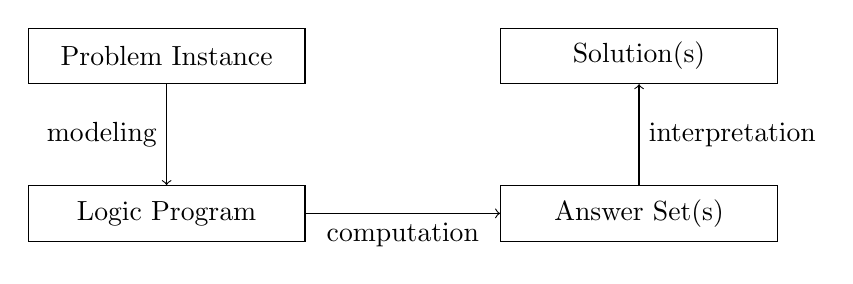
\begin{tikzpicture}
\tikzstyle{state} = [
 draw,
 minimum height=2em,
 minimum width=10em
]
\node[state] at (0,2) (i) {Problem Instance};
\node[state] at (0,0) (p) {Logic Program};
\node[state] at (6,0) (r) {Answer Set(s)};
\node[state] at (6,2) (s) {Solution(s)};

\path[draw,->] (i) -> node[left]{modeling} (p);
\path[draw,->] (p) -> node[below]{computation} (r);
\path[draw,->] (r) -> node[right]{interpretation} (s);
\end{tikzpicture}
  \end{center}
  \caption{High-level approach of using Answer Set Programming for declarative problem solving.}
  \label{fig:ASP1}
\end{figure}
 
Traditional answer set systems work in two phases:
\begin{enumerate}
\item Grounding: Given a program \(P\) with variables, a (subset) \(P'\) of its grounding is generated which has the same answer sets as \(P\).
\item Solving: The answer sets of the grounded (propositional) program \(P'\) are computed. First a candidate model is generated and then stability condition is checked.
\end{enumerate}

Different techniques have been developed over the years; DLV \cite{dlv}, Smodels \cite{smodels}, Platypus \cite{platypus} and clasp \cite{clasp} are example of solvers. Also, some systems avoid the \emph{grounding bottleneck} and interleave grounding and solving: ASPeRiX \cite{asperix,fofchain}, OMiGA \cite{omiga}, and Alpha, the system used in this work. For a more detailed explanation, refer to~\cite{primer,aspbook}.

\subsection{HEX-Programs}
HEX-programs~\cite{hex}, \emph{\underline{h}igher-order} logic programs with \emph{\underline{ex}ternal} atoms were introduced as a generalization of extended logic programs under the stable model semantics based on HiLog \cite{hilog}. The syntax of HEX-programs extend ordinary ASP programs by \emph{external atoms}, which enable a bidirectional interaction between a program and external sources of computation. External atoms have a list of input parameters and a list of output parameters. Informally, to evaluate an external atom, the reasoner passes the instantiated input parameters to the external source associated with the external atom. The external source computes output tuples that are matched with the output list. Formally, an external atom is of the form \(\&g[\vec{Y}](\vec{X})\), where \(\vec{Y} = Y_1, \dotso , Y_k\) are input parameters (from the set of terms, variables and predicates) and \(\vec{X} = X_1, \dotso , X_l \) are output terms.

Note that since predicate symbols may occur as input, this yields a higher order formalism. Implementations of external sources may consider the partial interpretation for input predicates at the time of evaluation.

A way to translate HEX-programs into (usual) first order programs by means of a polynomial reduction \(\Lambda(P)\) is given in \cite{hex}: (1.) Higher order atoms of the form \(Y_0(Y_1, \dotso, Y_n)\) are replaced by an ordinary atom \(a_n(Y_0, Y_1, \dotso, Y_n)\). A one-to-one correspondence between stable models of \(\Lambda(P)\) and \(P\) can be shown. (2.) External atoms require a more intricate treatment. We replace external atoms of the form \(\&g[\vec{X}](\vec{Y})\) by \(p_{\&g}(\vec{X},\vec{Y})\), but in the presence of negation as failure or non-monotone external atoms, more machinery is needed which we omit for brevity. For further details on the evaluation of HEX-programs refer to \cite{effeval1,effeval2}.
\section{The \ah agent}
\label{sec:agent}
% Describe the Angry Birds scenario/setting and how the agent works
\ah is an artificial player for Angry
Birds, which reasoning with respect to
the world knowledge is carried out by
means of computing the answer set of a
HEX-program.
It originated as a re-implementation of
the naive agent provided by the organizers
of the Angry Birds AI Competition~\cite{angryAI},
with general improvements on main components
of it and a complete rewriting of the
\emph{planning} component as a collection
of HEX-programs.

In this section, an overview of the \ah
agent will be presented, with a focus on
the declarative part and its features. 
For a full and detailed explanation of
the implementing process, of the agent
layout and additional considerations on
performance, the reader can refer to~\cite{angryhex}.

\subsection{Base Framework}

The Base Framework, upon which \ah is built,
consists of several modules, dealing with
different aspects of the game, from 
the interaction with the game environment,
provided by the \emph{Angry Birds} browser
extension and the \emph{Proxy} component of
the \emph{Game Server}, to the communication
between the agent client and the server,
mediated through the server/client \emph{Communication Port};
the following list describes the parts of main interest:
\begin{description}
    \item[Vision] This module segments the images
    captured from the game environment, returning
    the minimum bounding rectangles of essential
    objects, as well as relevant information,
    like the types of birds available, the material
    of which bricks are composed and where pigs are placed.
    \item[Trajectory] This component estimates
    the trajectory followed by a bird after being
    released; here, orientation and distance of 
    the release point with respect to the slingshot
    are taken into account.
    \item[Planning] also called \emph{AI agent} in the
    original setting, this part delivers the order
    of the played levels, the choice of birds to use
    and other strategy-related choices.
\end{description}

\subsection{Interaction with HEX-programs}

The main contribution brought by \ah is
found in the planning component, which has
been rewritten as a collection of HEX-programs.
These are partitioned in two layers, namely
the \emph{Tactic} and the \emph{Strategy} layer.
Then, these programs are feeded to the
\textsc{dlv-hex} solver~\cite{dlvHEX},
which returns answer sets containing
information about the next moves in the game.
\section{Complex Predicates~vs.~Complex Objects}
\label{sec:main}

In this section we present how a specific class occurences of higher order predicates can be translated to first order by introducing more complex terms.

For example, consider the following rule taken from the tactics of \ah:

% https://github.com/DeMaCS-UNICAL/Angry-HEX/blob/4ea72273518dfde6240ece9dadea927fd1b79c3c/dlv/tactic.dlv#L133

$$ canPush(o_a,o_b) :- \&canPush[objects,hills](o_a,o_b). $$

Intuitively, $canPush(o_a, o_b)$ should be true if the object $o_a$ can push the object $o_b$, which requires some minimum distance and geometric range.

Note that $objects$ and $hills$ are predicates, and in turn $\&canPush$ is a higher order predicate. We observe that $objects$ and $hills$ characterize the set of objects present in the current level of the game and the structure of the ground in the game respectively.

Since 

% How did we come up with the translation? Discovery of the translation.
% End to end example of translation for a predicate in \ah
\section{Conclusion}
\label{sec:conc}

In this work, we have shown how an ASP program, employing some features of a particular system, can be ported to another, by trading higher-order expressivity with more articulated term interpretations.
Specifically, we considered the \ah agent, described in~\cite{angryhex}, which underlying ASP system was \textsc{dlv-hex}; in order to port it to the \al solver, a higher-order elimination was needed.
The proposed translation achieves this result, by introducing Java classes as interpretations for terms.

Our implementation that results from the translation process covers all external atoms used by \ah, but since \al does not support weighted literals (allowing for optimization) rules using them were dropped. The source code is available at \url{https://github.com/lorenzleutgeb/angry-alpha}.

% How is this related to second order quantifier elimination? The universal closure over the rules with 2nd order predicates that we are elminiating should need second order quantifiers. After our translation process, they are gone. Have we just done second order quantifier elimination?

% Basically, we have reinvented lists as terms.

\bibliography{ref}
\end{document}
